\scanpage{73}
% archive sheet number: 72

\[
\underline{G}(k')\handwritten{\longrightarrow}\underline{G}(k)\ .
\]
The latter makes commutative \inserted{(modulo canonical isomorphism)}\handwritten{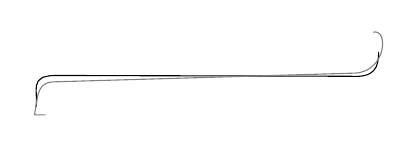
\begin{tikzpicture}[x=1cm,y=1cm,baseline=0cm]\draw[thin] (0,-.35)..controls (.03,-.15) and (-.1,.05)..(.25,.05)--(4,.04)..controls (4.3,.02) and (4.35,.15)..(4.35,.35);\draw[gray,thin] (.12,-.45)--(-.02,-.45)..controls (.03,-.15) and (.02,-.03)..(.26,-.03)--(4.05,.08)..controls (4.45,.1) and (4.48,.65)..(4.28,.6);\end{tikzpicture}} the diagram
\diagram{\begin{tikzcd}[ampersand replacement=\&,column sep=large,row sep=large]
\underline{G}(k\handwritten{'}) \handwritten{\arrow[r]} \handwritten{\arrow[d,draw=none,"{
\begin{tikzpicture}[x=1cm,y=1cm,baseline=0cm]\draw[thick] (0,.7)--(.025,-.5)..controls (.02,-.62) and (-.1,-.63)..(-.08,-.53);\fill (-.035,-.56) circle (.035);\end{tikzpicture}}" description]} \& \underline{G}(k^{\deleted{\unsure{'}}}) \handwritten{\arrow[d,draw=none,"{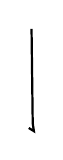
\begin{tikzpicture}[x=1cm,y=1cm,baseline=0cm]\draw[thick] (0,.7)--(.015,-.5)--(.03,-.6)--(-.035,-.56);\end{tikzpicture}}" description]} \\
\handwritten{\underline{\pi}_{p}}(k')\mathrm{x}\handwritten{[}G_m\handwritten{]}_{\underline{\unsure{\mathbb{Q}|Q}}_p} \handwritten{\arrow[r]} \& \handwritten{\underline{\unsure{\pi|\Pi}}}_p(k)\mathrm{x}\handwritten{[}\underline{G}_m\handwritten{]}_{\underline{Q}_p}
\end{tikzcd}}
(i.e. we have, on the corresponding Tannakian categories\deleted{, a}, a diag\unsure{\deleted{r}g|\deleted{g}r}am comm\unsure{\deleted{u}y|\deleted{y}u}tative up to \inserted{canonical}\handwritten{\begin{tikzpicture}[x=1cm,y=1cm,baseline=0cm]\draw[thin] (0,-.25)..controls (.12,.12) and (.3,.2)..(.6,.28)..controls (.9,.35) and (1.1,.4)..(1.18,.62);\end{tikzpicture}} isomorphism).

Forgetting in the latter the factors 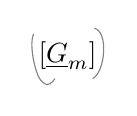
\begin{tikzpicture}[baseline=(f.base),x=1cm,y=1cm]\node[inner sep=0pt] (f) {$\handwritten{[}\underline{G}_m\handwritten{]}$};\draw[gray,thin] (-.43,.28)..controls (-.5,.14) and (-.4,-.3)..(-.31,-.34)..controls (-.24,-.4) and (-.2,-.34)..(-.16,-.29);\draw[gray,thin] (.34,.35)..controls (.52,.31) and (.48,-.2)..(.32,-.29);\end{tikzpicture}, we thus see that $\underline{G}(k')\handwritten{\longrightarrow}\underline{G}(k)$ factors through the sub-\deleted{category} gerbe of $\underline{G}(k)$ corresponding to the closed subgroup of $\handwritten{\pi}_1(k)$ image of $\handwritten{\pi}_1(k')$ ... To prove:

\uline{Proposition} \handwritten{6.1.} If $k'$ is an \deleted{finite} étale extension of $k$, then the homomorphism of gerbes $\underline{G}(k')\handwritten{\longrightarrow}\underline{G}(k)$ is a \uline{monomorphism} whose image is exactly the ``open'' sub-gerbe defined above. In particula\unsure{\deleted{r}t|\deleted{t}r}, if $k'$ is a finite Galois extension of $k$, \deleted{we have a} with \raisebox{.4ex}{G}alois group $g$, and we a canonical exact sequence of gerbes
\[
0\handwritten{\longrightarrow}\underset{\handwritten{\unsure{\mu|\deleted{\mu}|\pi|\deleted{\pi}}}}{\underline{G}^{\deleted{\unsure{'}}}}(k\handwritten{'})\handwritten{\longrightarrow}\underline{G}(k)\handwritten{\mathrel{\begin{tikzpicture}[baseline=0cm,x=1cm,y=1cm]\draw[thick] (0,0)--(.6,0);\draw[thick] (.55,0)--(.55,-.04);\end{tikzpicture}}}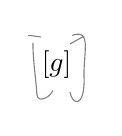
\begin{tikzpicture}[baseline=(f.base),x=1cm,y=1cm]\node[inner sep=0pt] (f) {$\handwritten{[}g\handwritten{]}$};\draw[gray,thin] (-.2,.35)--(-.36,.37);\draw[gray,thin] (-.3,.27)..controls (-.3,.04) and (-.26,-.2)..(-.25,-.38)..controls (-.24,-.51) and (-.06,-.4)..(-.05,-.33);\draw[gray,thin] (.2,.37)..controls (.46,.46) and (.33,.12)..(.35,-.2)..controls (.35,-.55) and (.2,-.52)..(.17,-.35);\draw[gray,thin] (.17,.26)--(.35,.36);\end{tikzpicture}_{\underline{Q}_p}\handwritten{\longrightarrow}0\ .
\]
This statement should be formally equivalent to the following: $\operatorname{Spec}(k')\handwritten{\longrightarrow}\operatorname{Spec}(k)$ is a morphism of effective descent for the fibred category of the $\mathrm{Fcriso}(L)$ over finite composites\inserted{$L$}\handwritten{\begin{tikzpicture}[x=1cm,y=1cm,baseline=0cm]\draw[thin] (0,-.3)..controls (.01,.02) and (.33,.3)..(.5,.48)..controls (.68,.65) and (.8,.74)..(.74,.88);\end{tikzpicture}} of fields of characteristic $p$. The proof of this last fact is $\handwritten{\pm}$ trivial.

\uline{Question} \handwritten{6.2.} Do we still have an analogous statement when we suppose that $k'$ is a Galois extension of $k$ which may be infinite ? The most interesting case would be that where $k'$is the separable closure of $k$, so that we would have a dévissage of $\underline{G}(k)$ into
\[
0\handwritten{\longrightarrow}\underline{G}(\handwritten{\bar{k}}^{\deleted{\unsure{'}}})\handwritten{\longrightarrow}\underline{G}(k)\handwritten{\longrightarrow\underline{\unsure{\pi|\Pi}}}_p(k)\handwritten{\longrightarrow}0\quad\deleted{\unsure{?}}\ ;
\tag*{\handwritten{(\unsure{6}.2.1)}}
\]
when $k$ is perfect i.e. $\handwritten{\bar{k}}$ algebraically closed, we shall see that $\underline{G}(\handwritten{\bar{k}})$ does not depend essentially on \handwritten{$k$. To}

\mspage{72}
